\chapter{Higgs Boson Physics}
\label{chap:higgs}
% The SM has been extremely successful in making predictions that were later confirmed by experimental measurements. Examples are the observation of the $W$ and $Z$ bosons in 1983 by the UA1 and UA2 collaborations, or the top quark discovery in 1995 by the CDF and D0 experiments. \todo{Maybe references}
% The observation of the $W$ and $Z$ bosons by the UA1 and UA2 collaborations in 1983 are just two examples of this.
% The discovery of the long sought-after Higgs boson in 2012 by the ATLAS and CMS collaborations~\cite{Aad:2012tfa,Chatrchyan:2012xdj} marks the highlight of this success story. 
% The success story culminated in the discovery of a new particle by the ATLAS and CMS collaborations in 2012~\cite{HIGG-2012-27,CMS-HIG-12-028}. To date, ten years after this discovery, the experimental evidence is overwhelming that the observed particle is the long sought-after Higgs boson predicted by the SM.

The new particle discovered in 2012 is now commonly referred to as the Higgs boson, since all measurements made so far have been consistent with the Higgs boson predicted by the SM.
However, the uncertainties on many of the measurements are still sizeable and much remains to be understood. 

The Higgs boson plays a special role in the SM. 
It is the only fundamental particle with a spin of zero and connected to a large fraction of the free parameters of the SM (see \cref{subsec:final-lagrangian}). It is also the only boson that is not a consequence of the principle of local gauge invariance, but arises from the ad-hoc introduction of EWSB via a scalar doublet field. 
Its unique nature makes the Higgs boson a prime candidate for searching for physics beyond the SM and thus relevant to many of the open fundamental questions~\cite{2019BHeinemann}. 
Some dark matter models, for example, predict interactions of the Higgs boson with yet unknown particles that are candidates for dark matter~\cite{Baumgart_2009,Kaplan_2009,Dienes_2012}. 
Other models such as two-Higgs-doublet models~\cite{Branco_2012} hypothesize the existence of additional particles similar to the Higgs boson as well as deviations from the SM predictions. 
These are important reasons for making precision measurements of the Higgs sector to test the predictions of the SM with ever-increasing precision.
This provides stringent constraints on models beyond the SM and may reveal deviations from the SM that could prove to be a gateway to discovering new physics. 

%This year (2022) marks the ten years anniversary of the Higgs boson discovery which is celebrated with a paper \cite{NaturePaper} that summarizes all state-of-the art Higgs measurements.
%The paper demonstrates that the observation of the Higgs in 2012 was only the beginning of an era, the era of Higgs precision measurements.
This section provides an overview of the phenomenology of Higgs boson processes. \Cref{subsec:higgschannels} summarizes the different production and decay modes of the Higgs boson, and \cref{subsec:exp-accessibility} discusses their experimental accessibility at the LHC. \Cref{subsec:xsec-measurements} outlines the different types of Higgs production cross-section measurements, before \cref{subsec:higgs-exp-status} concludes with a brief overview of the experimental status of Higgs physics at the time of writing.
%Many more details on the status of Higgs boson physics can be found in \cref{PDG2020}.

% From PDG:
% All these BSM scenarios can have important effects on the phenomenology of the Higgs boson.


% So far, there is no indication of deviations from the SM. 
% - Properties of the Higgs boson in agreement with the spin-parity JP = 0+ predicted by the SM. 
% - Cross sections all in agreement with the SM predictions. Firmly establishing VBF production in this thesis.
% - There is no indication that the found particle is not the SM. 
%The contrary, the experimental evidence is overwhelming that the measured particle is indeed the particle predicted by the SM.

% Wikipedia
%Since the Higgs field is scalar, the Higgs boson has no spin. The Higgs boson is also its own antiparticle, is CP-even, and has zero electric and color charge.[163]
% The Standard Model spin-parity JP = 0+
% \subsection{The role of the Higgs boson in the SM}
% \todo{Maybe add such a section -> Look for resources first!}

% \subsection{Motivation for Higgs physics}
% The Higgs boson plays a special role in the SM. 
% It is the only fundamental particle with a spin of zero and connected to a large fraction of the free parameters of the SM (see \cref{subsec:final-lagrangian}). 
% It is also the only boson that is not a consequence of the principle of local gauge invariance, but is added in an ad-hoc solution in the mechanism of EWSB. 
% Furthermore, the Higgs boson is a prime candidate for searching for physics beyond the SM and thus relevant to many of the open fundamental questions \cite{2019BHeinemann}.\footnote{This includes, for example, the search for dark matter (e.g. \ccite{Baumgart_2009,Kaplan_2009,Dienes_2012}) by testing models that predict interactions of the Higgs boson with yet unknown particles that are candidates for dark matter; or investigations of the process of EWSB itself by testing two-Higgs-doublet models~\cite{Branco_2012} that predict the existence of additional particles similar to the Higgs boson.}
% %\cite{2019BHeinemann} 

% The above-mentioned provides important reasons for performing precision measurements of the Higgs sector to test the predictions of the SM at an ever greater statistical precision and thus providing stringent constraints on models beyond the SM.
% Only with a precise knowledge of Higgs processes and an understanding of what exact role the Higgs boson plays in nature, fundamental physics can come closer to answering some of the open fundamental questions.  

% Precisely measuring the properties and cross sections of the Higgs boson is needed in order to understand the exact role it plays in nature and thus getting closer to answering some of the open fundamental questions. 

% From gianotti
% o gain even deeper insights into the Higgs boson and its role in fundamental physics

%OR: Precisely measuring the properties and cross sections of the Higgs boson is needed in order to understand the exact role it plays in nature and thus getting closer to answering some of the open fundamental questions. 

% From nature
% The measurements of those production and decay rates probe the strength of the interactions between the Higgs boson and the particles involved. This allows a test of an essential prediction of the SM: that the interaction strengths scale with particle masses.

% provide stringent constraints on many models of new phenomena beyond the Standard Model.


\section{Higgs boson production and decay modes}
\label{subsec:higgschannels}
The Higgs boson directly couples to all massive particles and therefore has various production and decay modes.
The relative contribution of the various modes (or \emph{channels}) are dependent on the mass of the Higgs boson, 
which was determined with a precision of less than 0.2\% in the most recent combined measurement by the ATLAS and CMS collaboration~\cite{HIGG-2014-14}.
%is determined to be $m_H=125.09 \pm 0.21(stat.) \pm 0.11(syst.)\,\GeV$ . 
%This offers a rich field of experimental signatures that can be explored by experiments.

\paragraph{Production modes} The Higgs production cross sections depend on the center-of-mass energy of the collider.
At the LHC, the four production modes illustrated in \cref{fig:higgsprodfeyn} dominate.
Their corresponding cross sections are shown in \cref{fig:higgsprodxsec}.
% \emph{gluon fusion} (ggF), \emph{vector-boson fusion} (VBF), \emph{Higgs-strahlung} from $W$ or $Z$ boson (VH), and $t\bar{t}$ fusion (ttH).
%- as illustrated in \cref{fig:higgsprodfeyn} with a choice of Feynman diagrams.
%associated production with a $t\bar{t}$ pair (also called \emph{$t\bar{t}$ fusion})
The \emph{gluon fusion} (ggF) process is the leading mechanism at the LHC and characterized by a virtual fermion loop coupling to the Higgs boson and no additional object in the final state (therefore labelled as $pp\rightarrow H$). 
The fermions in the loop are dominated by top-quarks because of their high mass. 
%The ggF cross section is calculated with an effective theory to NNNLO in QCD and includes electroweak corrections at NLO precision \cite{Anastasiou:2016cez}.\todo{double-check}
The second-largest contribution to Higgs boson production comes from the \emph{vector-boson fusion} (VBF) process, where two incoming quarks radiate a vector boson that fuse into the Higgs.
A main characteristic of the VBF production mode is the two quarks in the final state that appear at large angle and with a large invariant mass ($pp\rightarrow qqH$).
%The VBF Two quarks at large radii and with large invariant mass in the final state.
% This feature can be exploited to distinguish between collision events and select the subsequent decays of the Higgs boson. 
% In addition, the VBF production mode provides information about the couplings of the Higgs boson to the $W$ and $Z$ bosons. 
%Observation of the VBF production mode of the Higgs boson was found by a combined measurement of the ATLAS and CMS collaborations\cite{Khachatryan:2016vau}.
The \emph{Higgs-strahlung} process from $W$ or $Z$ bosons ($VH$) exhibits similar features, having one additional vector boson besides the Higgs boson in the final state ($pp \rightarrow WH$ and $pp \rightarrow ZH$).
The $t\bar{t}$ \emph{fusion} ($ttH$) process where the Higgs is produced in association with a $t\bar{t}$ pair is difficult to measure due to the relatively low production cross section and the less distinct final state ($pp \rightarrow ttH$). It plays an important role in Higgs boson physics, however, since it allows to directly measure the Yukawa coupling of the top quark. 
%The most recent results of the ATLAS collaboration yield evidence for the $t\bar{t}$-fusion production of the Higgs boson \cite{ATLAS-CONF-2017-077}.
The Higgs boson production in association with a $b\bar{b}$ pair ($pp\rightarrow bbH$) or a single-top quark ($pp \rightarrow tH$) have small contributions at the LHC, but are still contributing in combined measurements.

\paragraph{Decay modes}
Once the Higgs boson is produced, it decays almost instantaneously with a lifetime of about $10^{-22}$ seconds \cite{PDG2020}.
Therefore, only its decay products can be measured.
As discussed in \cref{sec:sm}, the coupling between the Higgs boson and the vector bosons (fermions) is predicted to be proportional to the squared mass of the vector bosons (the mass of the fermions). The resulting \emph{branching fractions} of the most relevant decays are displayed in \cref{fig:higgsbr}. 
The decay to a pair of bottom quarks ($H\rightarrow b\bar{b}$) is the leading process followed by the $H\rightarrow WW^*$ decay mode. Since the mass of the Higgs boson is lower than the summed mass of two $\Wpm$ or $Z$ bosons, the decay to vector bosons is suppressed and one of the decaying vector bosons appears as a virtual particle\footnote{Virtual particles have the same properties as on-shell particles, but can violate momentum and energy conservation for a short period limited by the uncertainty principle.}. The decay to other particles occurs significantly less often; some of the decay modes nonetheless produce detector signatures that are very suitable for studying the Higgs boson, as explained below.

\captionsetup[subfloat]{captionskip=10pt} % space between subfloat caption and image
\begin{figure}
  \begin{center}
    \subfloat[]{
      % use valgin if pie chart is shown for decays
      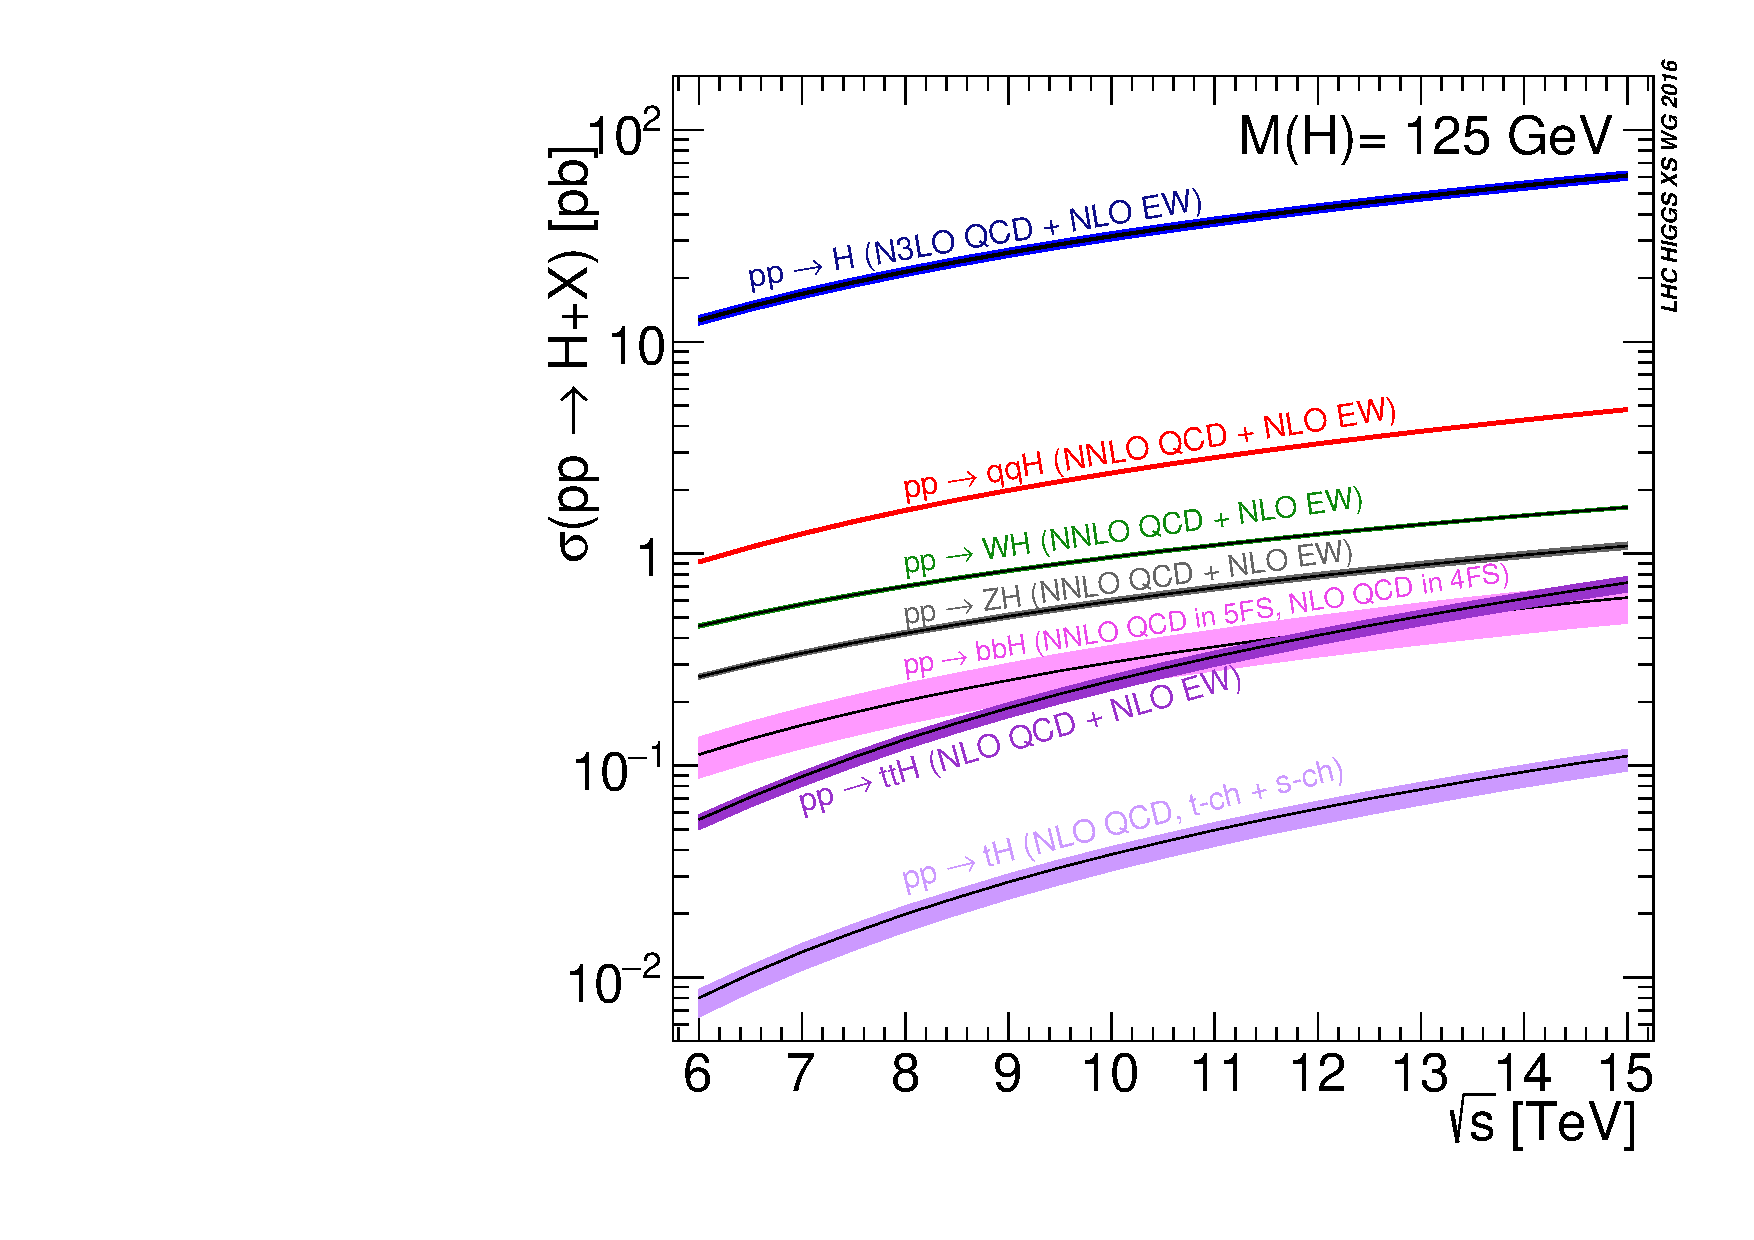
\includegraphics[scale=0.37]{figures/theory/Higgs_Prod_XSec_orig.pdf}
      \label{fig:higgsprodxsec}
    }
    % \hspace{-5em}
    % \captionsetup[subfloat]{captionskip=50pt} % space between subfloat caption and image
    % \subfloat[]{
    %   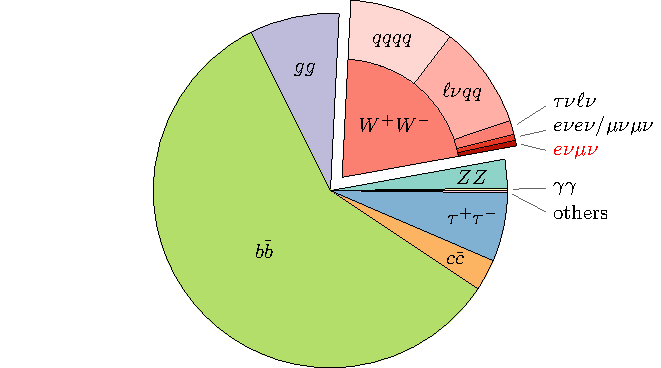
\includegraphics[scale=0.8,valign=t]{figures/theory/h-decay-pie/h-decay-pie.pdf}
    %   \label{fig:higgsbr}
    % }
        \subfloat[]{
            \newImageScale{figures/theory/SMHiggsBR_orig.pdf}{0.37}
            \label{fig:higgsbr}
          }
  \end{center}
  \caption{(a) Higgs boson production cross sections as a function of the LHC center-of-mass energy and (b) branching fractions of the Higgs boson. Taken from Ref.~\cite{deFlorian:2016spz}.}
  % \caption{(a) Higgs boson production cross sections as a function of the LHC center-of-mass energy. The line widths represent the respective theory uncertainties. Taken from Ref.~\cite{deFlorian:2016spz}. (b) branching fractions of the Higgs boson for a mass of 125\,\GeV. Values taken from Ref.~\cite{PDG2020}.}
  %  \label{fig:higgsbr}
\end{figure}
\captionsetup[subfloat]{captionskip=5pt} % space between subfloat caption and image

\captionsetup[subfloat]{captionskip=25pt} % space between subfloat caption and image
\unitlength=1mm
\begin{figure}
  \centering
\subfloat[Gluon fusion]{  
\begin{fmffile}{\feyndir/HiggsProduction_GluonFusion}
\begin{fmfgraph*}(60,22) 
\fmfleft{i1,i2}
\fmfright{o1,o2,o3}
\fmf{phantom}{i1,v1,o1} 
\fmffreeze 
\fmf{phantom}{i2,v2,o3}
\fmffreeze
\fmf{gluon, label=$g$, label.dist=+12.0}{i1,v1} 
\fmf{gluon, label=$g$, label.dist=+12.0}{i2,v2}
\fmf{fermion, label=$t$, label.dist=-12.0}{v1,v2,v3,v1}
\fmf{dashes, label=$H$,plain}{v3,o2}
\end{fmfgraph*}
\end{fmffile}
}
\quad
\subfloat[Vector-boson fusion]{
\begin{fmffile}{\feyndir/HiggsProduction_VBF}
\begin{fmfgraph*}(60,25) 
\fmfleft{i1,i2}
\fmfright{o1,o2,o3}
\fmf{phantom}{i1,v1,o1}
\fmffreeze
\fmf{phantom}{i2,v2,o3}
\fmffreeze
\fmfstraight
\fmf{phantom}{v1,v3,v2}
\fmffreeze
\fmf{fermion, label=$q$}{i1,v1}
\fmf{fermion, label=$q$}{i2,v2}
\fmf{fermion, label=$q^\prime$}{v1,o1}
\fmf{fermion, label=$q^\prime$}{v2,o3}
\fmf{boson, label=$W/Z$}{v1,v3,v2}
\fmffreeze 
\fmf{dashes, label=$H$,plain}{v3,o2}
\end{fmfgraph*}
\end{fmffile}
}
\\
\vskip1em
\subfloat[Higgs-strahlung]{
\begin{fmffile}{\feyndir/HiggsProduction_HiggsStrahlung} 
\begin{fmfgraph*}(60,25) 
\fmfleft{i1,i2}
\fmfright{o1,o2}
\fmf{fermion, label=$q$}{i1,v1}
\fmf{fermion, label=$q'$}{v1,i2}
\fmf{boson, label=$W/Z$}{v1,v2,o1}
\fmf{dashes, label=$H$}{v2,o2}
\end{fmfgraph*}
\end{fmffile}
}
\quad
\subfloat[$t\bar{t}$ fusion]{
\begin{fmffile}{\feyndir/HiggsProduction_ttbar}
\begin{fmfgraph*}(60,25) 
\fmfleft{i1,i2}
\fmfright{o1,o2,o3}
\fmf{phantom}{i1,v1,o1}
\fmffreeze
\fmf{phantom}{i2,v2,o3}
\fmffreeze
\fmfstraight
\fmf{phantom}{v1,v3,v2}
\fmffreeze
\fmf{gluon, label=$g$, label.dist=+12.0}{i1,v1}
\fmf{gluon, label=$g$, label.dist=+12.0}{i2,v2}
\fmf{fermion, label=$t$}{o3,v2,v3,v1,o1}
\fmf{dashes, label=$H$,plain}{v3,o2}
\end{fmfgraph*}
\end{fmffile}
}
\caption{Representative Feynman diagrams for the four main production modes of the Higgs boson at the LHC.}
\label{fig:higgsprodfeyn}
\end{figure}
\captionsetup[subfloat]{captionskip=5pt} % space between subfloat caption and image


\section{Experimental sensitivity of Higgs production at the LHC}
\label{subsec:exp-accessibility}
% From PDG
%For a given mH, the sensitivity of a channel depends on the production cross section of the Higgs
% boson, its decay branching fraction, the reconstructed mass resolution, the selection efficiency and
% the level of background in the final state. For a low-mass Higgs boson (110 GeV < mH < 150 GeV)
% for which the SM width would be only a few MeV, five decay channels play an important role
% at the LHC. In the H → γγ and H → ZZ∗ → 4` channels, all final state particles can be
% very precisely measured and the reconstructed mH resolution is excellent (typically 1-2%). While
% the H → W+W− → ` +ν`` 0−ν¯`
% 0 channel has relatively large branching fraction, however, due
% to the presence of neutrinos which are not reconstructed in the final state, the mH resolution,
% obtained through observables sensitive to the Higgs boson mass such as the transverse mass, is poor
% (approximately 20%). The H → b ¯b and the H → τ +τ
% − channels suffer from large backgrounds and
% lead to an intermediate mass resolution of about 10% and 15% respectively.

% PDG
% In order to optimize search sensitivity and also to separate the various Higgs
% boson production modes, ATLAS and CMS split events into several mutually exclusive categories

% For phrasing from PDG
% None of the other production modes have been firmly established by the experiments
% individually. However, the table shows that, for the VBF production mode, the combination had a
% large sensitivity and produced a combined observation of 5.4σ, therefore establishing this process
% with a rate compatible with that expected in the SM.

Physics analyses typically focus on a combination of production and decay mode (typically referred to as \emph{signal}) to measure the number of Higgs bosons produced. The experimental sensitivity of a particular channel is not only dependent on the respective production cross section and decay branching fraction, but also highly impacted by the signature of the final state. The final state signature determines, for example, how efficient the signal can be reconstructed in the ATLAS detector and how well it can be distinguished from other non-Higgs processes. 
%The different processes are typically first analyzed separately and then combined to obtain the most accurate measurements possible.

%and how well it can be distinguished from other types of events at hadron colliders. 
The $H\rightarrow b\bar{b}$ decay accounts for 58\% of all Higgs boson decays, but the experimental sensitivity to measure this decay mode is limited. The reason is the purely hadronic final state of $H\rightarrow b\bar{b}$ decays, which makes it difficult to distinguish the Higgs boson events from QCD multijet events that are abundant at the LHC.
%from the overwhelming background of QCD events at the LHC. 
The VBF or Higgs-strahlung production modes are therefore typically used where the presence of the additional particles in the final state can be exploited in the event selection.
%It is nonetheless possible to measure this decay by using the VBF or Higgs-strahlung production mode and 
%Using this strategy evidence for the $H\rightarrow b\bar{b}$ decay was recently found in the VH production mode \cite{Aaboud:2017xsd,Sirunyan:2017elk}.\todo{UPDATE}

The most sensitive channels for the Higgs boson discovery in 2012 were the Higgs boson decays to two photons ($H \to \gamma\gamma$), the $H \to ZZ^* \to llll$, and \HWW\ process.
%Higgs boson initially was discovered in the decay to two photons and the $H \rightarrow ZZ^* \rightarrow llll$ channel \todo{REF}.
The first two channels have relatively small branching fractions but exhibit very clean final-state signatures due to the presence of leptons and photons that can be very precisely measured and allow for a good handle over the background.
In addition, the mass of the Higgs boson can be fully reconstructed in these channels by computing the invariant mass of the reconstructed decay products.
%at a hadron collider, where an overwhelming fraction of events is dominated by QCD effects.
%This is equally important since it allows an excellent selection of signal events and a good control over the background. 
% the largest fraction of events are dominated by QCD effects.
%QCD dominated events
%events at a hadron collider, since the final states are dominated by QCD effects.
The \HWW\ decay also provides a good handle over the background when selecting leptonically decaying $W$ bosons.
The neutrinos stemming from the $W$ boson decays, however, prevent to fully reconstruct the mass of the Higgs boson, since they cannot be directly detected by the ATLAS experiment.

% Results of the analysis of \HWW\ decays conducted by the ATLAS collaboration and CMS collaboration for data of \RunOne\ can be found in Ref.~\cite{PhysRevD.92.012006} and Ref.~\cite{2013arXiv1312.1129C}, respectively; a corresponding analysis of \RunTwo\ data is given in \cref{sec:ggfanalysis}, focusing on the gluon fusion production-mode.

Events with $H \to \tau\tau $ decays exhibit a similar final state as the \HWW\ process and especially in the case of leptonically decaying $\tau$-leptons allows for an excellent background rejection. 
% htautau paper: https://arxiv.org/abs/2201.08269

The analyses of Higgs boson decays to second generation fermions are challenging, either because of very small branching fractions, as is the case for $H \to \mu\mu$ decays, or because of an overwhelming QCD background, as is the case for $H \to c\bar{c}$ decays.
% 125 considerably more challenging measurements of Higgs boson couplings to second-generation fermions are
% explored via searches for the 𝐻 → 𝜇+𝜇 −
% [32] and, for the first time, 𝐻 → 𝑐𝑐¯ [33] decays.
% From nature:
% The considerably more challenging measurements of Higgs boson couplings to second-generation fermions are explored via searches for the 𝐻 → 𝜇+𝜇−[32] and, for the first time, 𝐻 → 𝑐𝑐¯ [33] decays. Due to the large multijet background, the latter decay mode is currently accessed only via the 𝑊𝐻 and 𝑍𝐻 production. Finally, the inputs to the combination are complemented by the latest direct searches for Higgs boson decays into invisible particles which escape the detector undetected [34, 35].
%Latest cross-section measurements can be found in \todo{REF. Not sure if it's necessary}
%A similar final state as the one in \HWW\ processes, can be exploited when looking at Higgs boson decays into $\tau$-leptons \cite{Aad:2015vsa,Sirunyan:2276465}. 
The Higgs boson decays to $Z\gamma$ ($H \to Z\gamma$) are also very rare and therefore provide limited sensitivity to perform Higgs measurements.
% , where leptonically decaying $Z$ bosons provide the most sensible final state, or $\mu\mu$,  % \cite{Aaboud:2017uhw,Aaboud:2017ojs}.
The final states with gluons ($H \to gg$) make up a considerable fraction of all Higgs decays but are too difficult to differentiate from other events at the LHC.


\section{Higgs boson cross-section measurements}
\label{subsec:xsec-measurements}
% From PDG
% For a given mH, the sensitivity of a channel depends on the production cross section of the Higgs boson, its decay branching fraction, the reconstructed mass resolution, the selection efficiency and

% From Peskin/Schroeder
% The experiments that probe the behavior of elementary particles especially in the relativistic regime are scattering experiments. One collides two beams of particles with well dened momenta and observes what comes out The likelihood of any particular final state can be expressed in terms of the cross section, a quantity that is intrinsic to the colliding particles and therefore
% allows comparison of two dierent experiments with dierent b eam sizes and intensities


% From PDG
% In order to optimize search sensitivity and also to separate the various Higgs
% boson production modes, ATLAS and CMS split events into several mutually exclusive categories
The expected cross sections per production mode can be calculated from the SM Lagrangian, once the Higgs mass is fixed.
Since the total decay width of the Higgs boson ($\approx 4\,\MeV$~\cite{deFlorian:2016spz}) is much smaller than its mass, the narrow-width approximation holds, which allows measuring the Higgs cross sections as a product of the production cross section times the branching fractions of the decay modes.
For a given process with final state $Y$, the number of observed Higgs boson events is typically expressed in terms of a \emph{signal strength}, defined as 
\begin{equation}
  \label{eq:signal-strength}
  \mu(pp \to H \to Y) = \frac{ [ \sigma(pp \to H)  \times \BR(H \to Y) ]_\text{meas} } { [ \sigma(pp \to H) \times \BR(H \to Y) ]_\text{SM}},
\end{equation}
where the subscript ``meas'' (``SM'') denotes the measured value (prediction of the SM), and $B$ denotes the branching fraction. 
The following briefly outlines the different types of cross-section measurements that are performed in the field of Higgs boson physics. 

% This allows, for example, measuring cross sections in exclusive regions of phase space which improves the resolution with which SM predictions can be probed.
%Differential measurements also allow for easier interpretability of the results, for example in Effective Field Theories (EFT) \todo{REF}.

\subsubsection{Inclusive production cross-section measurements}
Historically, the first measurements of the Higgs boson were based on the total amount of Higgs bosons produced per production mode.
These inclusive production mode cross sections are maximally dependent on theoretical assumptions related to the decay properties of the Higgs boson.
They are typically conducted for the search of a new signal (as done for the Higgs discovery in 2012) or to experimentally establish different production modes in the SM.
However, inclusive measurements cannot resolve small deviations from the SM predictions that may occur in regions of phase space where only a small fraction of the total produced Higgs bosons are expected.

\subsubsection{Differential cross-section measurements}
%As more data has been collected at the LHC in recent years, 
In order to probe the SM predictions at a greater resolution, Higgs production processes can be measured differentially in various kinematic and topological variables.
Differential measurements use well-defined measurement regions, known as \emph{fiducial regions}, that allow unfolding the detector effects. 
This enables comparisons between experimental data and theory at generator level and thus minimizes the dependency on theoretical assumptions. 
Due to the rather complex unfolding procedure, the use of advanced analysis techniques such as neural networks is discouraged, which limits the sensitivity of differential measurements.
Another drawback is that it is not easily possible to statistically combine differential measurements with different definitions of the fiducial region.  

% - Least theory dependent
% - Not easily possible to combine measurements, as unfolding procedure very tailored to analysis selection. 

\subsubsection{Simplified template cross section measurements}
The \emph{Simplified Template Cross Sections} (STXS) framework provides a way to maximize experimental sensitivity while still allowing for differential measurements of Higgs boson production.
To achieve this, mutually exclusive kinematic regions of Higgs boson production are defined, based purely on the production mode and kinematics of the Higgs boson and agnostic to the different Higgs decay channels. The kinematic regions that are often referred to as \emph{STXS bins} are defined at generator level and agreed upon between experiments.
These design choices allow combining Higgs measurements of different decay channels as well as experiments, which enables more precise cross-section measurements.
% The measurements of the production mode cross sections are performed in regions of phase space defined at the level of the fully reconstructed collision events. They are defined as similar as possible to the generator-level bins. This allows using sophisticated analysis techniques like neural networks.
The specific bins are chosen following two main principles: First, the experimental acceptance is aimed at being constant within each bin, which reduces the dependency on theoretical assumptions. Second, regions that are expected to be sensitive to physics effects beyond the SM are isolated, so that they can be studied separately.
As the amount of available data increases, the STXS binning evolves in stages, each time increasing the number of bins. 

%% \begin{figure}
%%   \newImageScale{figures/Higgs_Prod_XSec.pdf}{0.5}
%%   \caption{Higgs boson production cross sections and their theory uncertainties for different values of the LHC centre of mass energy. \cite{YR4}}
%%   \label{fig:higgsprodxsec}
%% \end{figure}



% \subsection{Properties of HWW Decays}
% % THIS MIGHT actually fit in the analysis section
% % as it directly related to what analysis selections we perform
% % THINK ABOUT IT!
% - VBF Higgs -> ww cross section must be exactly the SM value, otherwise VBS xsec converges!
% -> Maybe add this to HWW analysis

\section{Current Experimental Status}
\label{subsec:higgs-exp-status}
% All experimentally accessible decay modes of the Higgs have been observed, which includes $H \to \gamma\gamma$, $H \to ZZ$, $H \to WW$, $H \to \tau\tau$, and $H \to b\bar{b}$. 
The data from \RunOne\ and \RunTwo\ of the LHC allowed for high-precision measurements of several properties of the Higgs boson such as its mass, spin, or parity, as well as Higgs boson production and decay processes. 
At the time of writing, all experimental measurements are consistent with the predictions of the SM.
This section briefly summarizes the current experimental status, mostly focusing on results of the ATLAS collaboration.
%allowing to place the work presented in this thesis into a broader context. 

\subsection{Higgs boson properties}
The latest combined measurement of the ATLAS and CMS experiment~\cite{HIGG-2014-14} measures a Higgs mass of 
\begin{equation}
  m_H = 125.09 \pm 0.21\text{(stat.)} \pm 0.11\text{(syst.)}\,\GeV.
\end{equation}
Analyses performed by the ATLAS and CMS collaboration using \RunTwo\ data measure a mass of $m_H = 124.97\pm0.28\,\GeV$~\cite{ATLAS-CONF-2017-046} and $m_H = 125.26 \pm 0.21\,\GeV$~\cite{Sirunyan_2020}, respectively.
Measurements of the spin and CP of the Higgs boson confirm the SM predictions of a spin-parity $J^P = 0^+$ and exclude alternative hypothesis beyond 99.9\% confidence level (CL).~\cite{HIGG-2013-17-witherratum,CMS-HIG-14-018} 

\subsection{Higgs production and decay processes}
All major Higgs boson production modes (ggF, VBF, $VH$, $ttH$) and Higgs boson decays to bosons ($H \to W^\pmW^\mp$, $H \to ZZ$, $H \to \gamma\gamma$) as well as third-generation fermions ($H \to \tau^+\tau^-$, $H \to b\bar{b}$) have been observed at the LHC with significances larger than $5\,\sigma$ above the background expectation.~\cite{NaturePaper}
While precision measurements are now being performed for these channels, rarer Higgs boson processes have not been confirmed with the data available. 
Experimental signs of the $H \to Z\gamma$ decay and decays to second-generation fermions ($H \to \mu^+\mu^-$, $H \to c\bar{c}$) are found in the data of \RunTwo of the LHC.~\cite{HIGG-2018-42,HIGG-2019-14,ATLAS-CONF-2021-021}.
Other decay modes predicted ($H \to s\bar{s}$; decays to first-generation fermions $H \to e^+e^-$, $H \to u\bar{u}$, $H \to d\bar{d}$; and decays to gluons $H \to gg$) remain experimentally inaccessible at the LHC. 

% A summary of the latest measurements performed by the ATLAS collaboration of the kinematic properties of Higgs boson production, as well as the Higgs boson's coupling to other particles can be found in \cref{NaturePaper}.
The latest Higgs boson measurements performed by the ATLAS collaboration are summarized in \cref{NaturePaper}.
%  They constitute the most precise measurements at the time of writing.
The results are based on a combination of several Higgs boson analyses, one of which is the \HWW\ analysis that is presented in detail in \cref{chap:hww} of this thesis. 
The remainder of this section summarizes the main results of the paper, which allows placing the measurements presented in this thesis in a broader context. 

% The following provides an overview of the experimental status of Higgs measurements at the time of writing, which allows placing the measurements presented in this thesis in a broader context. 
% ==>> Experimental status
% - Listing the most recent measurements?!
% - Give outline of current status of Higgs measurements, focusing on cross section measurements.
% - A more comprehensive and complete overview is given in \cref{PDG2020}..

\paragraph{Higgs production}
%%%%%%%%%%%%%%%%%%%%%%%%%%%%%%%%%%%%%%%
The fully inclusive Higgs boson signal strength is measured to be \cite{NaturePaper}
\begin{equation*}
   \mu =1.05 \pm 0.06 = 1.05\pm 0.03\, (\text{stat.})\, \pm 0.03\, (\text{exp.})\, \pm 0.04\, (\text{sig.\ th.})\, \pm 0.02\, (\text{bkg.\ th.}),
\end{equation*}
when assuming that all production and decay processes scale with the same signal strength $\mu$.

%%%%%%%%%%%%%%%%%%%%%%%%%%%%%%%%%%%%%%%
% Prod mode cross section
The cross sections of the different Higgs production modes times the branching fraction are measured for specific combinations of production and decay processes. 
The results are shown in \cref{fig:prod-per-channel} and reveal the precision with which different Higgs boson processes have been measured to date. 
The analysis of \HWW\ decays is among the most precise measurements in particular for the ggF and VBF production mode.
%As can be seen, 
\begin{figure}
  \newImageResizeCustom{1}{figures/theory/higgs-measurements/fig4.pdf}
  \caption{Ratio of observed rate to predicted SM event rate for different combinations of
  Higgs boson production and decay processes. The horizontal bar on each point denotes the 68\% confidence interval. The narrow grey bands indicate the theory uncertainties in the SM cross section times the branching
fraction predictions. The $p$-value for compatibility of the measurement and the SM prediction is
72\%. Figure and caption taken from \ccite{NaturePaper}.}
  \label{fig:prod-per-channel}
\end{figure}
%%%%%%%%%%%%%%%%%%%%%%%%%%%%%%%%%%%%%%%%%%
% Decay fractions
% \todo{Maybe putting the decay fraction results is not necessary here!}
% The Higgs decay branching fractions can be measured by fixing the production mode cross section to the respective SM expectation and assuming that there are no non-SM decays. The results can be seen in \cref{fig:br-per-channel}.
%%%%%%%%%%%%%%%%%%%%%%%%%%%%%%%%%%%%%%%%%%
% - Latest STXS combination (from nature)
The results of the Higgs boson production mode cross-sections measured in several kinematic regions are shown in \cref{fig:stxs-stage12}. The region partitioning follows the so-called Stage 1.2 STXS scheme. 
The classification of Higgs boson production into 5 classes ($t\bar{t}H$, $tH$, $qq\to Hqq$, $pp\to VH$, and $gg\to H$) is detailed in \cite{NaturePaper}. 
% From nature paper
% Higgs boson production is first classified according to the nature of the initial state and the associated particles, the latter including the decay products of $W$ and $Z$ bosons if they are present. These classes are: $t\bar{t}H$ and $tH$ processes; $qq'\to Hqq'$ processes, with contributions from both VBF and quark-initiated $VH$ (where $V=W, Z$) production with a hadronic decay of the vector boson; $pp\to VH$ production with a leptonic decay of the vector boson ($V(\ell\ell,\ell\nu)H$), including $gg\to ZH \to \ell\ell H$ production; and finally the ggF process combined with $gg\to ZH \to q\bar{q}H$ production to form a single $gg\to H$ process. The contribution of the $b\bar{b}H$ production process is taken into account as a $1\%$~\cite{YR4} increase of the \ggtoH\ yield in each kinematic region, since the acceptances for both processes are similar for all input analyses~\cite{YR4}.
% \Cref{fig:stxs-stage12} shows as an example the bins defined in Stage 1.2 of the STXS framework for Higgs measurements with two quarks in the final state ($pp \to qqH$), which is inclusive in Higgs bosons produced via VBF or quark-initiated $VH$ processes. 
% Different bins are defined for the number of jets in the event, as well as the transverse momentum of the Higgs, $p_T^{H}$, and the invariant mass of the dijet system, $m_{jj}$\footnote{The dijet system in a given event is typically defined by the two jets with largest transverse momentum}.
% %  A further splitting is performed based on the transverse momentum of the combined system of the Higgs boson and the two jets, labelled as $p_T^{Hjj}$. 

\begin{figure}
  \newImageResizeCustom{1}{figures/theory/higgs-measurements/fig8.pdf}
  \caption{Observed and predicted Higgs boson production cross sections in different
  kinematic regions. The vertical bar on each point denotes the 68\% confidence interval. The $p$-value for compatibility of the combined measurement and the SM prediction is 94\%. Kinematic regions are defined separately for each production process, based on the jet multiplicity, the transverse momentum of the Higgs ($p_{\textrm{T}}^H$) and vector bosons ($p_{\textrm{T}}^W$ and $p_{\textrm{T}}^Z$) and the two-jet invariant mass ($m_{jj}$).
The `VH-enriched' and `VBF-enriched' regions with the respective requirements of $m_{jj}\in[60, 120)$ \GeV\ and $m_{jj}\notin[60,120)$ \GeV\ are enhanced in signal events from $VH$ and VBF productions, respectively. Figure and caption taken from \ccite{NaturePaper}.
  }
  \label{fig:stxs-stage12}
\end{figure}

\paragraph{Higgs couplings}
The couplings of the Higgs boson to individual particles can be measured by parametrizing the cross section times branching fractions for the individual Higgs processes in terms of coupling-strength modifiers, $\kappa$, following the $\kappa$-framework \cite{LHCHandbookV3}. 
% For a production (decay) via the coupling to a given particle $p$, the modifier $\kappa_p$ is defined as $\kappa_p^2 = \sigma_p / \sigma_p^\text{SM}$ ($\kappa_p^2 = \Gamma_p/\Gamma_p^\text{SM}$), where $\Gamma_p$ is the partial decay width into a pair of particles $p$.\cite{NaturePaper}
%Different statistical models with varying assumptions that are detailed in \cite{NaturePaper} may be considered. 
Assuming that there are only SM processes that interact exactly as predicted, and independently measuring coupling strength modifiers for all included particles ($W$, $Z$, $t$, $b$, $c$, $\tau$, and $\mu$), the results can be visualized as shown in \cref{fig:h-couplings}. 
This finds good consistency of the internal structure of the SM, but at the same time reveals that the uncertainties on the measurements are still sizeable. 
If the measurement is performed using only two coupling-strength modifiers, one for the vector bosons, $\kappa_V = \kappa_W = \kappa_Z$, and one for all fermions, $\kappa_F$, the results are $\kappa_V = 1.035 \pm 0.031$ and $\kappa_F = 0.95 \pm 0.05$. 
%and Higgs boson to fermion coupling, $\kappa_{F}$, are measured with a relative uncertainty of the order of 10\% and 20\%, respectively. 

\begin{figure}
  \newImageResizeCustom{0.7}{figures/theory/higgs-measurements/fig6_paper.pdf}
  \caption{
    Reduced Higgs boson coupling strength modifiers and their uncertainties. They are defined as $\kappa_F \cdot m_F / \text{vev}$ for fermions
($F=t,b,\tau,\mu$) and $\sqrt{\kappa_V}\cdot m_V/\text{vev}$ for vector bosons as a
function of their masses $m_F$ and $m_V$. Two fit scenarios with $\kappa_c =
\kappa_t$ (colored circle markers), or $\kappa_c$ left free-floating in the fit (grey
cross markers) are shown. Loop-induced processes are assumed to have the SM structure, and Higgs boson decays to non-SM particles are not allowed. The vertical bar on each point denotes the 68\% confidence interval. The $p$-value for compatibility of the combined measurement and the SM prediction are 56\% and 65\% for the respective scenarios. The lower panel shows the values of the coupling strength modifiers. The grey arrow points in the direction of the best-fit value and the corresponding grey uncertainty bar extends beyond the lower panel range. Figure and caption taken from \ccite{NaturePaper}.}
  \label{fig:h-couplings}
\end{figure}

\paragraph{Searches for rare and invisible Higgs processes}
Rare decay modes of the Higgs boson have become experimentally accessible with data from \RunTwo\ of the LHC. 
The search for Higgs decays to a pair of muons found an excess of $H \to \mu\mu$ events over the background expectation of 2.0 standard deviations, where 1.7 were expected~\cite{HIGG-2019-14}.
The analysis of $H \to cc$ events yields an observed (expected) upper limit of 26 (31) times the SM prediction~\cite{ATLAS-CONF-2021-021}, and the search for $H \to Z\gamma$ decays results in an observed (expected) upper limit of 3.6 (2.6) times the SM prediction~\cite{HIGG-2018-42}.
An upper limit on the branching fraction of Higgs decays to particles that are invisible to the detector was set to 0.145, where 0.103 was expected~\cite{ATLASInvisible1}.
The cross section of di-Higgs production is extremely low. The most stringent upper limits by the ATLAS collaboration were set to 4.1 times the SM prediction at 95\% CL using $HH \to b\bar{b}\gamma\gamma$ decays~\cite{ATLAS-CONF-2021-016}.

%Other search to invisible: \cite{Aad_2022}

% From nature
% Even with the current precision of measurements there is room for possible interpretations of the data in terms of new phenomena beyond the SM. 

% From nature
% Finally, the inputs to the combination are complemented by the latest direct searches for Higgs boson
% 129 decays into invisible particles which escape the detector undetected [34, 35].

\TDinote{}{Add section on Differential Higgs measurement!}

\subsection{Effective field theories}
Measurements of Higgs production cross sections also serve as basis for further interpretation, for example within the framework of Standard Model Effective Field Theory (SMEFT)\footnote{An overview of SMEFT can, for example, be found in \ccite{}.}. In SMEFT, the effects of physics beyond the SM at large energy scales $\Lambda$ -- large compared to the Higgs vacuum expectation value ($\Lambda \gg v$) -- are parametrised at low energies, $E \ll \Lambda$, in terms of effective couplings. 
This allows for a theory-independent approach to search for deviations of the SM. 
Using a combination of different Higgs cross-section measurements, the ATLAS collaboration was able to put constraints on new physics~\cite{ATLAS-CONF-2020-053}.
As well, the ATLAS collaboration combined the analysis of \HWW\ decays with differential cross-section measurements of $WW^*$ production in order to interpret the measured cross sections in terms of effective couplings~\cite{ATL-PHYS-PUB-2021-010}.
Both of these results pave the way for future interpretations of Higgs measurements in effective field theories, which become especially important in the absence of any direct discovery of new particles. 

% % The latest combined Higgs measurements performed by the ATLAS collaboration of the kinematic properties of Higgs boson production, as well as the Higgs coupling to other particles, are nicely summarized in \ccite{NaturePaper}.

% In addition to the results presented in \ccite{NaturePaper}, Higgs analyses can be interpreted in the framework of Effective Field Theories. 
% Effective field theories parametrise...
% They allow for a general parametrisation of deviations of the SM. 
% \todo{2-3 sentences on EFT.}

% %Differential measurements also allow for easier interpretability of the results, for example in Effective Field Theories (EFT).

